\documentclass[11pt, a4paper]{article}

\usepackage[margin=20mm]{geometry}
\usepackage[T2A]{fontenc}
\usepackage[utf8]{inputenc}
\usepackage[russian]{babel}
\usepackage{DejaVuSans}
\usepackage{DejaVuSansMono}
\renewcommand{\familydefault}{\sfdefault}

\usepackage{amsmath, amssymb}
\usepackage{graphicx}
\usepackage{booktabs}
\usepackage{xcolor}
\usepackage{tikz}
\usepackage{hyperref}
\usepackage{enumitem}

\definecolor{primary}{RGB}{30, 64, 175}
\definecolor{secondary}{RGB}{71, 85, 105}
\definecolor{lightbg}{RGB}{248, 250, 252}

\hypersetup{
	colorlinks=true,
	linkcolor=primary,
	urlcolor=primary
}

\pagestyle{plain}

\begin{document}

\begin{center}
    {\large \textbf{Практикум цифрового производства · Осень 2026}} \\[0.5em]
    {\LARGE \textbf{\color{primary} Предложение проекта}} \\[0.5em]
    {\huge \textbf{Дроид с интегрированной обработкой сенсорных данных и всенаправленной реакцией}} \\[1em]
    \textbf{Команда:} Матисов Егор, Бехтин Григорий, Кенунен Арсений (Группа Б03-505)
\end{center}

\vspace{0.5em}
\hrule
\vspace{1.5em}

% 1
\section{Введение и концепция проекта}
Современные мобильные робототехнические платформы требуют сочетания высоких показателей проходимости, автономности и интеллектуальности навигации. Данный проект посвящен разработке четвероногого шагающего робота (квадропода) с интегрированным грузовым отсеком и возможностью автономного выполнения навигационных задач внутри помещений.

Инновационность системы заключается в разделении вычислительных нагрузок между микроконтроллерной подсистемой реального времени (отвечающей за инверсную кинематику и стабилизацию) и высокоуровневым микрокомпьютером (осуществляющим обработку визуальных данных и сетевое взаимодействие).

% 2
\section{Цели и задачи проекта}

\subsection{Основная цель}
Спроектировать, собрать и отладить действующий прототип четырехногой шагающей платформы грузоподъемностью до 0.5~кг, способной по команде из Telegram-бота осуществлять автономное перемещение в заданную точку помещения, ориентируясь по данным технического зрения и массива ИК-датчиков, с последующим автоматическим возвратом на базовую зарядную станцию.

\subsection{Задачи проекта}
\begin{enumerate}[leftmargin=*]
    \item \textbf{Аппаратная разработка и CAD-проектирование:}
    \begin{itemize}
        \item Расчет механических нагрузок на суставы и определение необходимых крутящих моментов сервоприводов.
        \item 3D-моделирование элементов корпуса, сочленений и 3-DOF конечностей.
        \item Изготовление конструктивных компонентов методом аддитивного производства (3D-печать).
    \end{itemize}
    \item \textbf{Электронное конструирование:}
    \begin{itemize}
        \item Разработка двухуровневой вычислительной архитектуры (Raspberry Pi Zero 2 W + Arduino Uno + Servo Shield).
        \item Интеграция сенсорного массива: гироскоп/акселерометр (IMU), ИК-датчики расстояния, оптическая камера.
        \item Проектирование автоматизированной зарядной станции с направляющим ИК-маяком и упругими контактными площадками.
    \end{itemize}
    \item \textbf{Программное обеспечение и алгоритмы:}
    \begin{itemize}
        \item Реализация алгоритмов обратной кинематики (IK) и управление походкой дроида в реальном времени.
        \item Разработка алгоритмов локализации и распознавания меток на базе Python и OpenCV.
        \item Построение Telegram-бота для дистанционного управления и веб-интерфейса для отслеживания телеметрии и передачи видеопотока.
    \end{itemize}
\end{enumerate}

% 3
\section{Архитектура системы и кинематика}
Каждая из 4 конечностей платформы имеет 3 степени свободы (3 DOF), что позволяет позиционировать стопу в любой точке рабочего пространства в пределах допустимых углов поворота сервомоторов. Общее число управляемых степеней свободы робота равно 12.

\begin{figure}[!h]
    \centering
    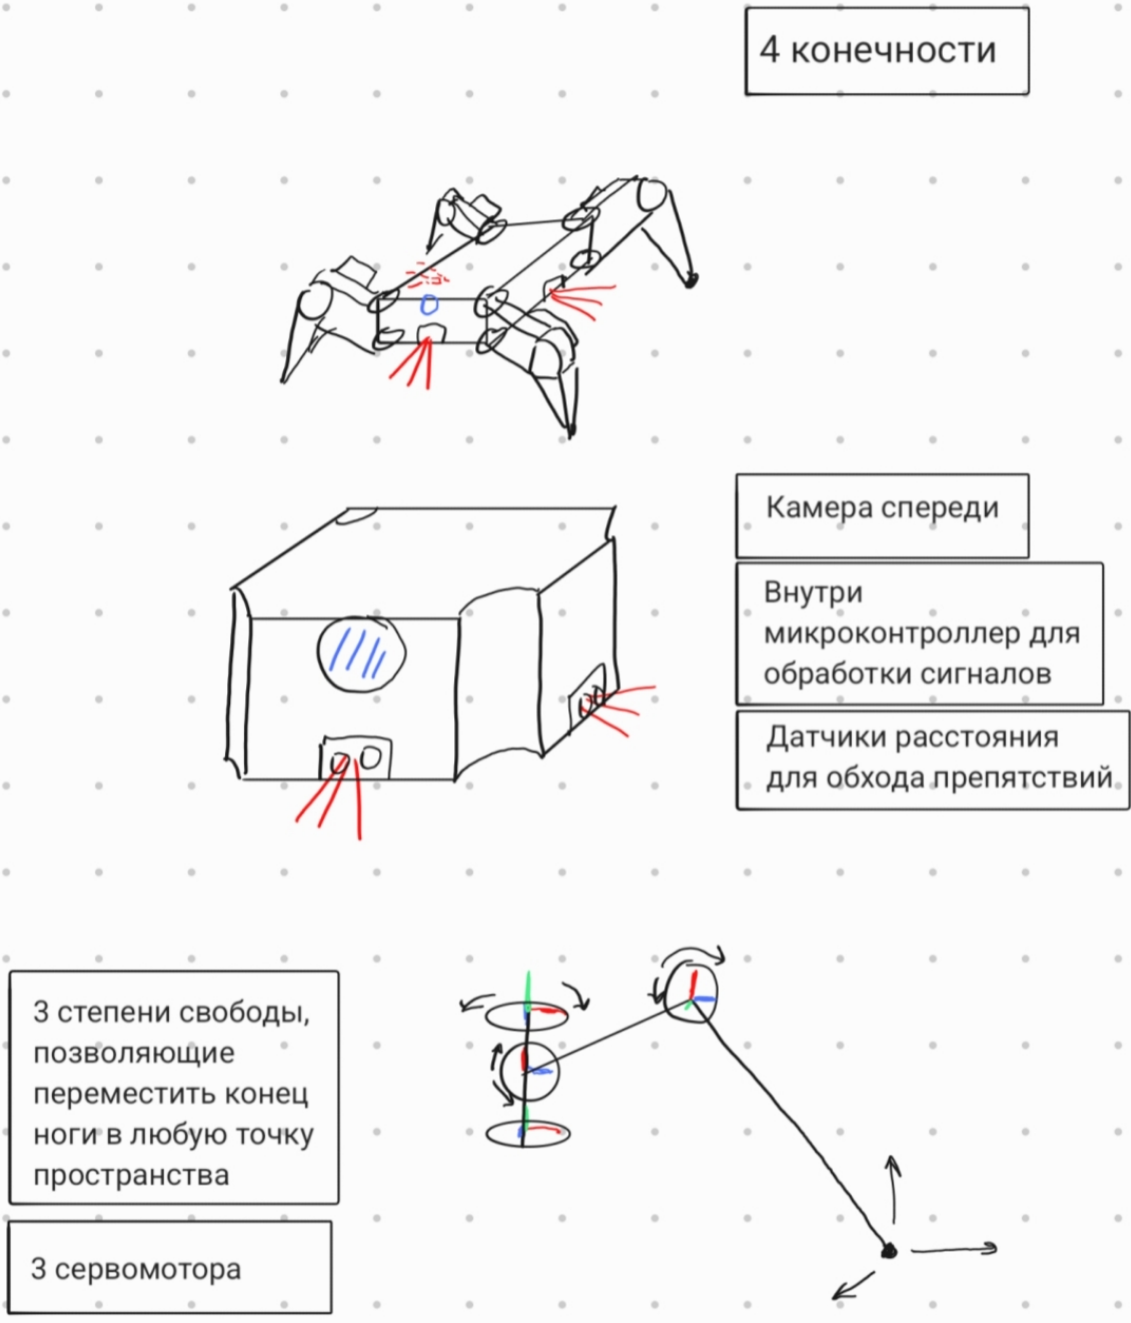
\includegraphics[width=0.6\textwidth]{схема.png}
    \caption{Эскизная схема расположения узлов и сенсоров шагающего дроида.}
    \label{fig:robot_sketch}
\end{figure}

% 4
\section{Программное обеспечение и алгоритмы}
Система управления состоит из двух ключевых уровней:
\begin{itemize}[leftmargin=*]
    \item \textbf{Низкоуровневый модуль (Arduino Uno):} отвечает за генерацию PWM-сигналов для 12 сервоприводов, опрос IMU-сенсора для динамической балансировки и первичную фильтрацию показаний ИК-датчиков расстояния.
    \item \textbf{Высокоуровневый модуль (Raspberry Pi Zero 2 W):} осуществляет обработку видеопотока с камеры $640\times640\text{p}$, распознавание ArUco/AprilTag маркеров, расчёт траектории движения, планирование обхода препятствий и взаимодействие с Telegram API.
\end{itemize}

% 5
\section{Анализ существующих аналогов}
В качестве базы для проведения исследований и проектирования кинематической схемы были рассмотрены следующие открытые проекты:
\begin{enumerate}[leftmargin=*]
    \item \textbf{SpotMicroAI:} Open-source клон робота Boston Dynamics Spot масштаба $\approx 30$ см на базе 12 сервоприводов. Из данного проекта заимствуются принципы построения кинематической модели и базовые алгоритмы формирования шага.
    \item \textbf{Quadruped Bionic Spider Robot Kit (ESP8266):} Модульный комплект робота-паука. Проанализированы подходы к компоновке корпуса и электропитанию.
\end{enumerate}

% 6
\section{Спецификация компонентов}

В таблице~\ref{tab:components} приведен перечень необходимых комплектующих для сборки прототипа дроида и базовой станции.

\begin{table}[h!]
    \centering
    \caption{Спецификация компонентов и элементов системы}
    \label{tab:components}
    \vspace{0.5em}
    \begin{tabular}{llc}
        \toprule
        \textbf{№} & \textbf{Наименование компонента} & \textbf{Количество} \\
        \midrule
        1 & Микроконтроллер Arduino Uno & 1 шт. \\
        2 & Одноплатный компьютер Raspberry Pi 3 Model B+ & 1 шт. \\
        3 & Сервопривод JX PDI-2010MG (высокий крутящий момент) & 4 шт. \\
        4 & Сервопривод Feetech FS90 & 8 шт. \\
        5 & Датчик расстояния ИК (5–50 мм) & 4 шт. \\
        6 & Оптическая камера ($640\times640\text{p}$) & 1 шт. \\
        7 & Servo Shield расширение для Arduino & 1 шт. \\
        8 & RGB Светодиод (индикация статуса) & 2 шт. \\
        9 & Монохромная LED матрица $8\times8$ (модуль) & 1 шт. \\
        10 & Модуль гироскопа и акселерометра (IMU) & 1 шт. \\
        11 & Комплект качалок и крепежа для сервомоторов & 4 комплекта \\
        \bottomrule
    \end{tabular}
\end{table}
	
\end{document}